\section{3Dスキャナ}
3Dスキャナは物体の形状を計測し, 3Dデータへと変換する装置である.
3Dスキャナには接触式や非接触式など, 複数の種類が存在し, 測定する物体に応じて使い分ける.
\figref{Fig:artecleo}のような非接触式3Dスキャナはレーザや光を使って物体の表面をスキャンし, そのデータを3次元点群に変換する.
非接触式の中でも, Artec Leoのような手で持って測定するものをハンディタイプといい, 測定する環境が狭い場合や, 測定したい物体が複雑な構造を持つ場合でも小回りがきくため, 細かい部分まで計測できるという利点がある.
3Dスキャナは, 品質検査やリバースエンジニアリング, 文化財等をデジタルアーカイブとして保存することなど, 幅広い分野で活用されており, 物体を3Dデータ化することができる.

\begin{figure}[H]
     \centering
     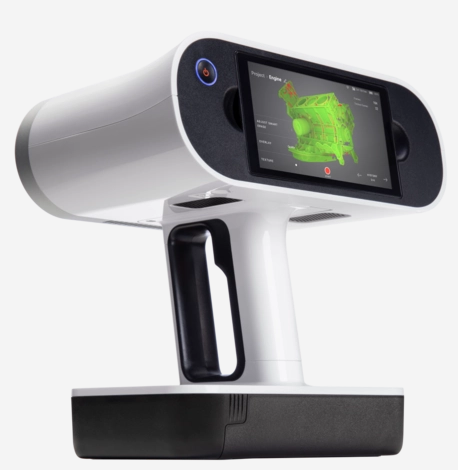
\includegraphics[width=50mm]{images/png/artecleo.png}
     \caption[Artec Leo]{Artec Leo (source: \cite{artecleo})}
     \label{Fig:artecleo}
   \end{figure}